\documentclass[french]{report}
\usepackage[utf8]{inputenc}
\usepackage[T1]{fontenc}
\usepackage[dvipsnames]{xcolor}
\usepackage{babel,hyperref,graphicx}

\hypersetup {
    colorlinks=true,
    linkcolor=black,
    urlcolor=blue,
}

\addto\captionsfrench{\renewcommand{\partname}{Méthode}}
\addto\captionsfrench{\renewcommand{\chaptername}{Partie}}

\makeatletter
\@addtoreset{chapter}{part}
\makeatother

\graphicspath{ {./resources/} }

\title {
    \Huge\bfseries Science des données \\
    \vskip .5em
    \large TP 1 – Iris
    \vskip 1.5em
}
\author {
    Taillieu Victor \\ \textit{21 154 689}
    \and
    Vaio Luca \\ \textit{21 154 698}
}
\date{\vskip 1em\today}

\begin{document}
    \maketitle
    \tableofcontents
    
    \setlength{\parskip}{1em}
    
    \chapter*{Introduction}
    \addcontentsline{toc}{chapter}{Introduction}
    
    Les concepts et techniques permettant de comprendre, visualiser et séparer des données sont multiples.
    À travers ce TP, nous allons explorer des données en combinant ces différents outils afin d'acquérir une bonne capacité d'analyse et une maîtrise des techniques utilisées.
    L'objectif étant de montrer le mieux possible la séparation entre plusieurs classes d'un jeu de données.
    
    Celui qui est utilisé pour ce TP est Iris : \url{https://archive.ics.uci.edu/ml/datasets/iris}.
    Il contient 150 observations réparties en trois classes (\texttt{setosa}, \texttt{versicolor} et \texttt{virginica}) de 50 observations chacune.
    Les attributs décrivant ces observations sont au nombre de quatre : \texttt{sepal\_length}, \texttt{sepal\_width}, \texttt{petal\_length} et \texttt{petal\_width}.
    Les classes d'Iris sont relativement bien séparées dans l'espace à quatre dimensions.
    Nous devons donc montrer que ces classes sont en effet bien distinctes dans un espace plus réduit de une à deux dimensions.
    
    Pour commencer, nous tenterons de présenter cette séparation en se basant sur des fonctions de séparation et des mesures de distance.
    Enfin, nous utiliserons une approche plus visuelle à travers des figures de nuages de points ou d'histogrammes avec ou sans transformation des données initiales.
    
    
    \part{Calcul de distances}
    \chapter*{Objectifs de cette méthode}
    
    Avec cette première méthode, nous cherchons à montrer la séparation entre les différentes classes des données d'Iris grâce à des fonctions de séparation.
    Celles-ci permettent d'obtenir des mesures quantitatives indiquant l'écart entre les observations.
    
    Ici, nous nous concentrerons sur des mesures de distance et de qualité de classe que sont la distance euclidienne, la distance de Mahalanobis, la distance intra-classe (cohésion) et la distance inter-classe (séparation).
    
    \noindent Notre démarche pour cette méthode est la suivante :
    
    \begin{itemize}
        \item Implémenter les différentes fonctions de distance
        \item Calculer les distances intra et inter-classe en utilisant les distances euclidienne et de Mahalanobis pour chaque paire de classe
        \item Répéter l'étape précédente en normalisant les données
        \item Tester différentes combinaisons de variables pour les calculs de distance
    \end{itemize}
    
    \chapter{Distances spatiales}
    
    \section{Cohésion et séparation}
    
    \paragraph{Cohésion}
    La distance intra-classe (ou cohésion) représente la distance maximale entre un objet quelconque d'une classe \texttt{A} et le centre de cette classe.
    Autrement dit, c'est le plus grand écart entre la moyenne de la classe et un point de celle-ci.
    
    \paragraph{Séparation}
    La distance inter-classe (ou séparation) est quant à elle définie comme étant la distance minimale entre un objet quelconque d'une classe \texttt{A} et le centre de la classe \texttt{B}.
    Il s'agit donc du plus petit écart entre la moyenne de la classe \texttt{B} et un point de la classe \texttt{A}.
    
    \paragraph{}
    Par déduction, si la distance intra-classe est inférieure à la distance inter-classe, alors on peut conclure que les classes en question sont bien séparées.
    En effet, cela signifie qu'il n'y a pas de point de la classe \texttt{A} plus proche du centre de la classe \texttt{B} que n'importe quel point de la classe \texttt{B}.
    
    \section{Mesures de distance}
    
    \subsection{Distance euclidienne}
    La distance euclidienne entre deux vecteurs $u$ et $v$ est caractérisée par le carré de la différence de leurs composantes, comme le montre la formule suivante :
    \begin{equation}
        \mathrm{dist}(u,v)=\sqrt{\sum_{k=1}^d(u_k-v_k)^2}
    \end{equation}
    
    \noindent C'est en fait un cas particulier de la distance de Minkowski, qui est la suivante :
    \begin{equation}
        \mathrm{dist}(u,v)=\sqrt[L]{\sum_{k=1}^d|u_k-v_k|^L}
    \end{equation}
    
    
    \subsection{Distance de Mahalanobis}
    La distance de Mahalanobis est quand à elle caractérisée par la formule suivante :
    \begin{equation}
        \mathrm{dist}(u,v)=(u-v)^T\cdot\Sigma^{-1}\cdot(u-v)
    \end{equation}
    
    \noindent Où $\Sigma$ est la matrice de variance-covariance de l'ensemble de données $X$ :
    \begin{equation}
        \Sigma=\frac1{n-1}\sum_{i=1}^n(x_i-\mu)\cdot(x_i-\mu)^T
    \end{equation}
    
    \paragraph{}
    La principale différence entre ces deux mesures de distance est que la distance de Mahalanobis tient compte de la forme de dispersion des données.
    Par exemple elle détecte les formes allongées de type elliptique alors que la distance euclidienne se contente des formes de type sphérique.
    
    \chapter{Résultats}
    
    \section{Distance euclidienne}
    
    La formule de la distance euclidienne est assez simple et son calcul est direct.
    Elle prend en paramètres deux observations (sous forme de vecteurs) puis retourne un nombre réel représentant la distance séparant ces deux objets.
    
    Il y a différentes façons d'appliquer la distance euclidienne.
    En effet, il est possible de ne sélectionner qu'un sous-ensemble des attributs des objets.
    Dans notre cas, il y a quatre attributs (\texttt{sepal\_length}, \texttt{sepal\_width}, \texttt{petal\_length} et \texttt{petal\_width}).
    Il est donc possible de choisir n'importe quelle combinaison de ces variables.
    
    Pour chaque paire de classe, calculons donc la distance intra-classe de la première puis la distance inter-classe entre les deux classes.
    Ce calcul est effectué dans les deux sens car la distance inter-classe est directionnelle (de la classe 2 à la classe 1).
    Le calcul de ces distances en utilisant la formule d'Euclide avec les quatre variables donne les résultats suivants :
    
    \begin{table}[h]
        \centering
        \begin{tabular}{||c c c c c||}
            \hline
            \textbf{Classe 1} & \textbf{Classe 2} & \textbf{Intra-classe} & \textbf{Inter-classe} & \textbf{Séparées} \\
            \hline\hline
            setosa & versicolor & 1.25 & 1.99 & {\color{ForestGreen}oui} \\
            setosa & virginica & 1.25 & 3.50 & {\color{ForestGreen}oui} \\
            \hline
            versicolor & setosa & 1.55 & 2.86 & {\color{ForestGreen}oui} \\
            versicolor & virginica & 1.55 & 0.76 & {\color{BrickRed}non} \\
            \hline
            virginica & setosa & 2.07 & 4.34 & {\color{ForestGreen}oui} \\
            virginica & versicolor & 2.07 & 0.65 & {\color{BrickRed}non} \\
            \hline
        \end{tabular}
        \caption{Distances selon la formule euclidienne.}
    \end{table}
    \leavevmode
    
    D'après le tableau ci-dessus, les distances inter-classe sont supérieures aux distances intra-classe pour toutes les paires contenant \texttt{setosa}.
    Ainsi, on peut en conclure que la classe \texttt{setosa} est bien séparée des classes \texttt{versicolor} et \texttt{virginica}.
    Cependant, nous ne pouvons pas affirmer que les classes \texttt{versicolor} et \texttt{virginica} sont séparées en se basant sur ces résultats.
    
    Nous pouvons aller un peu plus loin en testant les différentes combinaisons possibles de variables comme énoncé plus haut.
    Il n'en résulte toutefois pas de meilleurs résultats, ils sont en fait soit similaires, soit moins bons.
    Nous pouvons néanmoins relever un point important : toutes les combinaisons contenant la variable \texttt{petal\_length} permettent de séparer la classe \texttt{setosa} des deux autres.
    Cet attribut est donc primordial dans la distinction de cette classe.
    Voici le tableau des résultats obtenus en utilisant uniquement \texttt{petal\_length} dans le calcul de la mesure de distance :
    
    \begin{table}[h]
        \centering
        \begin{tabular}{||c c c c c||}
            \hline
            \textbf{Classe 1} & \textbf{Classe 2} & \textbf{Intra-classe} & \textbf{Inter-classe} & \textbf{Séparées} \\
            \hline\hline
            setosa & versicolor & 0.46 & 1.54 & {\color{ForestGreen}oui} \\
            setosa & virginica & 0.46 & 3.04 & {\color{ForestGreen}oui} \\
            \hline
            versicolor & setosa & 1.26 & 2.36 & {\color{ForestGreen}oui} \\
            versicolor & virginica & 1.26 & 0.24 & {\color{BrickRed}non} \\
            \hline
            virginica & setosa & 1.35 & 3.65 & {\color{ForestGreen}oui} \\
            virginica & versicolor & 1.35 & 0.45 & {\color{BrickRed}non} \\
            \hline
        \end{tabular}
        \caption{Distances euclidiennes avec \texttt{petal\_length} seulement.}
    \end{table}
    
    \section{Distance de Mahalanobis}
    
    \subsection{Covariance globale}
    
    La distance de Mahalanobis permet un peu plus de flexibilité dans son calcul.
    En plus de devoir fournir les deux objets pour lesquels la distance les séparant doit être mesurée, on doit fournir une matrice de covariance.
    Ainsi, nous disposons d'un certain degré de liberté dans l'élaboration de cette matrice.
    
    Cette mesure de distance devrait être plus intéressante, pourtant après une première tentative, les résultats ne sont pas concluants.
    En utilisant l'ensemble des données pour calculer la matrice de covariance, toutes les classes se retrouvent non séparées selon les critères des distances intra et inter-classe vus plus haut.
    
    La méthode n'est en fait pas la bonne.
    Pour que la mesure de distance soit cohérente, la matrice de covariance doit être calculée sur la classe à partir de laquelle la mesure est effectuée.
    
    \subsection{Covariance par classe}
    
    L'idée est donc, par exemple pour le calcul de la distance intra-classe de \texttt{setosa} et inter-classe entre \texttt{setosa} et \texttt{versicolor}, de calculer la matrice de covariance sur les données de \texttt{setosa}.
    
    En suivant cette méthode, voici les résultats obtenus :
    
    \begin{table}[h]
        \centering
        \begin{tabular}{||c c c c c||}
            \hline
            \textbf{Classe 1} & \textbf{Classe 2} & \textbf{Intra-classe} & \textbf{Inter-classe} & \textbf{Séparées} \\
            \hline\hline
            setosa & versicolor & 3.51 & 11.65 & {\color{ForestGreen}oui} \\
            setosa & virginica & 3.51 & 20.94 & {\color{ForestGreen}oui} \\
            \hline
            versicolor & setosa & 3.53 & 7.31 & {\color{ForestGreen}oui} \\
            versicolor & virginica & 3.53 & 2.32 & {\color{BrickRed}non} \\
            \hline
            virginica & setosa & 3.70 & 11.11 & {\color{ForestGreen}oui} \\
            virginica & versicolor & 3.70 & 1.66 & {\color{BrickRed}non} \\
            \hline
        \end{tabular}
        \caption{Distances de Mahalanobis, covariances par classe.}
    \end{table}
    \leavevmode
    
    Nous avons donc réussi à séparer la classe \texttt{setosa} par rapport aux autres. Ensuite, comme pour la distance euclidienne, nous avons testé différentes combinaisons de variables et les résultats sont similaires, les classes séparées de la même manière.
    
    On constate également que la distance de Mahalanobis permet d'amplifier la distance inter-classe vis-à-vis de la distance intra-classe. Cela renforce l'aspect sépararé des classes par rapport à la distance euclidienne.
    
    Toutefois, malgré les différentes tentatives, les deux autres classes que sont \texttt{virginica} et \texttt{versicolor} n'ont pas pu être séparées en utilisant des fonctions de séparation.
    
    
    \part{Visualisation des données}
    \chapter*{Objectifs de cette méthode}
    
    Avec cette deuxième méthode, nous cherchons à visualiser la séparation entre les différentes classes des données d'Iris par des figures d'histogrammes (pour une variable) ou de nuages de points (pour deux variables).
    Les différents graphiques permettront d'observer les groupements de classe et de voir ou non leur séparation.
    
    Cette méthode est donc plutôt visuelle tandis que la première était quantitative.
    Nous travaillerons avec les variables issues du jeu de données original Iris ainsi que des transformations de ces dernière en utilisant l'analyse en composantes principales (ACP).
    
    \noindent Notre démarche pour cette méthode a été la suivante :
    
    \begin{itemize}
        \item Visualiser la distribution des classes par paire selon chaque variable
        \item Visualiser la distribution des classes par paire selon chaque composante principale
        \item Visualiser les nuages de points pour toutes combinaisons de deux variables
        \item Visualiser les nuages de points pour toutes combinaisons de deux composantes principales
    \end{itemize}
    
    \chapter{Visualisation univariée}
    
    \section{Données initiales}
    
    Pour cette première visualisation univariée, nous avons produit des histogrammes représentant la distribution de chaque variable et pour chaque paire de classes, ce qui donne 4 variables $\times$ 3 combinaisons de paires de classes = 12 visualisations.
    Nous avons choisi d'afficher ici, pour chaque paire, l'histogramme de la variable montrant le mieux la séparation entre les deux classes sélectionnées, en l'occurrence \texttt{petal\_length}.
    Lorsque les distributions se chevauchent, les barres sont affichées l'une par-dessus l'autre.
    
    \begin{figure}[h]
        \centering
        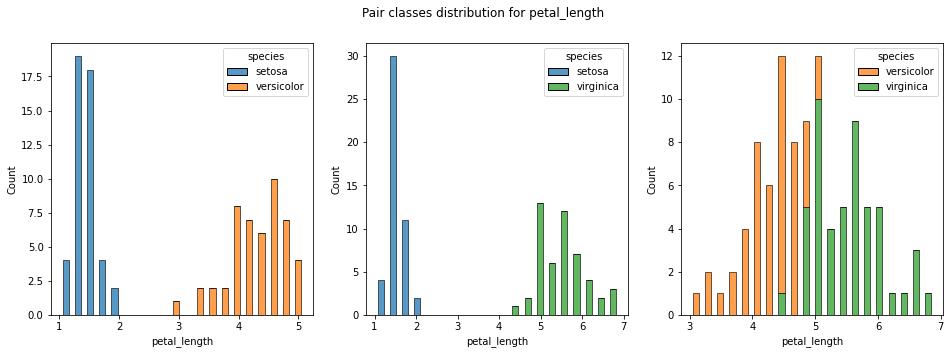
\includegraphics[width=\textwidth]{univar_raw_petal_length}
        \caption{Distribution des classes par paires pour \texttt{petal\_length}}
    \end{figure}
    
    On constate donc, comme attendu, que la classe \texttt{setosa} (en bleu) est clairement séparée des autres classes.
    Par contre, les classe \texttt{versicolor} et \texttt{virginica} se chevauchent sur un ensemble assez large de données.

    \section{Données avec transformation ACP}
    
    Nous avons ensuite réalisé la même démarche en appliquant cette fois-ci une analyse en composantes principales (ACP).
    Ainsi, nous obtenons quatre nouvelles variables, calculées à partir du jeu de données original et de quatre composantes principales.
    
    \subsection{Données initiales}
    
    À chaque composante principale est associée une valeur propre, qui représente le niveau d'explication de la variance des données par la composante correspondante.
    Commençons par travailler sur nos données brutes, voyons quelles sont les valeurs propres pour notre analyse ACP.
    
    \begin{table}[h]
        \centering
        \begin{tabular}{|c c c c|}
            \hline
            $\lambda_1$ & $\lambda_2$ & $\lambda_3$ & $\lambda_4$ \\
            \hline
            4.23 & 0.24 & 0.08 & 0.02 \\
            \hline
        \end{tabular}
    \end{table}
    
    La première valeur propre semble bien plus élevée que les autres, et en effet en voici la distribution :
    
    \begin{figure}[h]
        \centering
        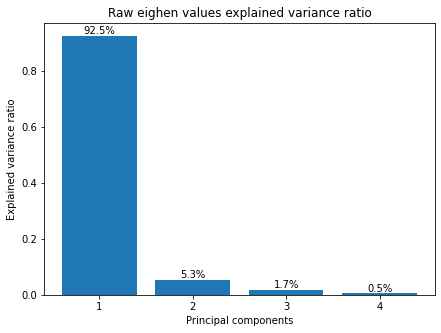
\includegraphics[width=0.75\textwidth]{raw_eighen_ratio}
        \caption{Distribution des valeurs propres, données initiales}
    \end{figure}
    \leavevmode
    
    De fait, c'est bien évidemment la composante principale \#1 qui permet le mieux de distinguer les paires de classes pour chaque combinaison (voir page suivante).
    
    \begin{figure}[h]
        \centering
        \includegraphics[width=\textwidth]{univar_full_pca_pairs}
        \caption{Distribution des classes selon la composante principale 1}
    \end{figure}
    
    On constate à nouveau sur ce graphe que les classes \texttt{versicolor} et \texttt{virginica} se chevauchent beaucoup.
    L'ACP n'a donc pas permis de séparer ces deux classes.
    
    Cependant, il reste encore une possibilité : plutôt que de faire l'analyse sur l'ensemble du jeu de données, il est possible que les composantes calculées sur une seule classe
    
    \subsection{Données normalisées}
    
    En procédant à l'ACP avec les données normalisées, la première valeur propre est moins prédominante, expliquant 73\% de la variance seulement.
    
    \begin{figure}[h]
        \centering
        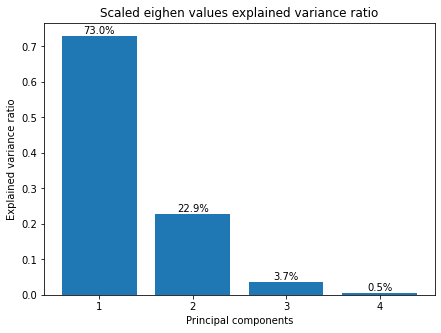
\includegraphics[width=0.69\textwidth]{raw_eighen_ratio_scaled}
        \caption{Distribution des valeurs propres, données normalisées}
    \end{figure}
    
    
    Cependant, la normalisation des donnée ne nous a pas permis non plus de clairement séparer les trois classes, peu importe les composantes choisies pour la projection.
    C'est pourquoi nous avons ensuite tenté d'appliquer l'analyse en composantes principales autrement.
    
    
    Dans cette section, plutôt que de déterminer les composantes sur l'ensemble du jeu de données, nous allons le faire sur chacune des trois classes \texttt{setosa}, \texttt{versicolor} et \texttt{virginica}.
    Ensuite seulement nous projetterons l'ensemble des données sur ces composantes.
    
    Le but de cette manipulation est de déterminer les vecteurs expliquant au mieux la variance d'une classe de données bien précise, ce qui semble finalement plus pertinent.
    
    Nous avons donc effectué l'analyse sur toutes les classes, à la fois avec les données brutes et les données normalisées.
    Cela ne nous a néanmoins pas permis de séparer les classes \texttt{versicolor} et \texttt{virginica}.
    
    Le meilleur résultat sur une dimension est obtenu sur \texttt{setosa}, avec les données normalisées, projeté sur la troisième composante.
    
    \begin{figure}[h]
        \centering
        \includegraphics[width=0.75\textwidth]{univar_pca_setosa_scaled}
        \caption{ACP sur \texttt{setosa}, données normalisées}
    \end{figure}
    
    
    \chapter{Visualisation bivariée}
    
    \section{Données initiales}
    
    Visualisons maintenant les classes selon deux variables sur des nuages de points.
    De la même façon, nous avons un total de 12 graphiques à visualiser.
    La meilleure façon de comparer la distribution des données selon chaque variable est de générer une grille de paires de variables, comme suit :
    
    \begin{figure}[h]
        \centering
        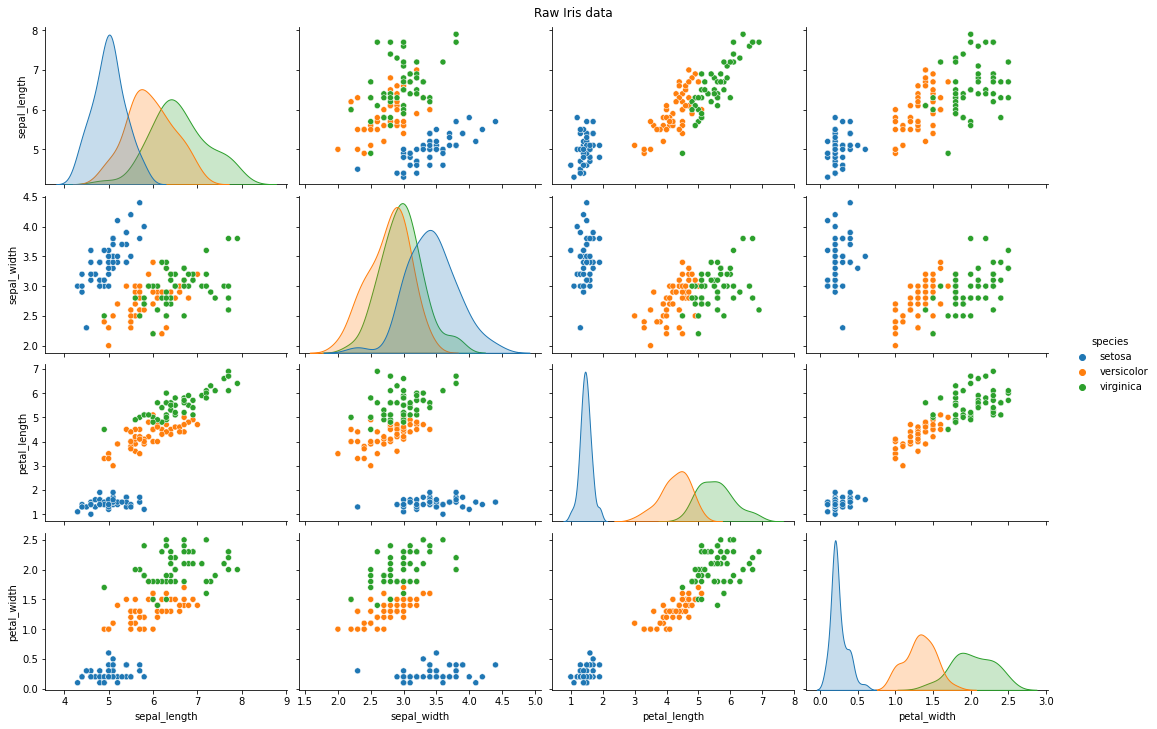
\includegraphics[width=\textwidth]{multivar_raw_full}
        \caption{Grille des données initiales selon chaque paire de variable}
    \end{figure}
    
    La meilleure visualisation est celle représentant les classes selon la longueur et la largeur de leurs pétales.
    
    \begin{figure}[h]
        \centering
        \includegraphics[width=0.75\textwidth]{multivar_raw}
        \caption{Données initiales selon \texttt{petal\_width} et \texttt{petal\_length}}
    \end{figure}
    
    Comme précédemment, on voit clairement la classe \texttt{setosa} se détacher des deux autres.
    Par contre, \texttt{virginica} et \texttt{versicolor} restent légèrement superposées.
    
    \section{Données avec transformation ACP}
    
    Pour finir, reprenons les transformations ACP effectuées précédemment afin d'afficher les résultats selon deux composantes cette fois.
    Après visualisation, nous constatons que la meilleure projection se fait sur les composantes 1 et 2.
    Les projections avec les composantes 3 ou 4 par contre sont inintéressantes.
    \newpage
    \begin{figure}[h]
        \centering
        \includegraphics[width=0.75\textwidth]{multivar_full_pca}
        \caption{Données transformées par ACP selon les composantes 1 et 2}
    \end{figure}
    \leavevmode
    
    Enfin, en appliquant l'ACP sur une seule classe, la meilleure visualisation semble être la projection sur les composantes 3 et 4, calculées avec \texttt{virginica}.
    Les trois classes, cependant, ne sont pas entièrement séparées.
    
    \begin{figure}[!h]
        \centering
        \includegraphics[width=0.75\textwidth]{multivar_pca_virginica_scaled}
        \caption{ACP sur \texttt{virginica} selon les composantes 4 et 3}
    \end{figure}
    
    \chapter*{Conclusion}
    \addcontentsline{toc}{chapter}{Conclusion}
    
    Pour conclure, nous avons vu deux méthodes permettant d'évaluer la séparation des données.
    
    D'abord par le calcul de distances, et nous avons vu que la distance de Mahalanobis est une approche plus précise lorsque la distribution est elliptique.
    
    Ensuite, par la visualisation, donc à une ou deux dimensions.
    La méthode ici est donc de projeter le jeu de données sur de nouveaux axes potentiellement plus propices à la compréhension de sa structure.
    
    Pour finir, les différentes visualisations ne nous ont pas permis de clairement séparer les trois classes, mais ce TP nous a permis d'appréhender différentes options de transformation des données qui semblent tout de même efficaces.
\end{document}
